%!TEX root = /Users/ego/Boulot/TKZ/tkz-fct/doc-fr/TKZdoc-fct-main.tex  
\subsection{Courbes de \tkzname{Van der Waals}}

\bigskip
Soient $v$  le volume  d'une masse fluide et  $p$ sa pression. 
$b$ et $k$ sont deux nombres réels strictement  positifs. On souhaite étudier une formule exprimant la dépendance de ces variables proposée par Van~der~Waals.
\[
  p(v)= \frac{-3}{v^2} + \dfrac{3k}{v-b}
\]

définie sur l'intervalle $I=\big]b~;~+\infty\big]$

\subsubsection{Tableau de variations}
\begin{center}
  
 \begin{tkzexample}[]  
  \begin{tikzpicture}
  \tkzTab%
  { $v$      /1,%
    $g'(v)$  /1,%
    $g(v)$   /3%
  }%
  { $b$ ,%
    $3b$ ,%
    $+\infty$%
  }%
  {0,$+$,$0$,$-$,t}
  {-/           $0$    /,%
   +/$\dfrac{8}{27b}$  /,%
   -/  $0$             /}%
  \end{tikzpicture}
\end{tkzexample}
\end{center}



\newpage

\subsubsection{ Première courbe avec  \emph{b}=1} 
 Quelques courbes pour $r\leq\ v \leq\ 6$ 

  

\medskip
\begin{center}
	\begin{tkzexample}[] 
	 \begin{tikzpicture}[xscale=2,yscale=2.5]
	    \tkzInit[xmin=0,xmax=6,ymax=0.5,ystep=0.1]
	    \tkzDrawX[label=$v$]
	    \tkzDrawY[label=$g(v)$]
	    \tkzGrid(0,0)(6,0.5)
	    \tkzFct[color   = red,domain =1:6]{(2*(x-1)*(x-1))/(x*x*x)}
	    \tkzDrawTangentLine[color=blue,draw](3)  
	    \tkzDefPointByFct(1)  
	    \tkzText[draw, fill = brown!30](4,0.1){$g(v)=2\dfrac{(v-1)^2}{v^3}$}
	 \end{tikzpicture} 
	\end{tkzexample} 
\end{center}


\newpage 
\subsubsection{ Deuxième courbe  \emph{b}=1/3 }   


\medskip
\begin{center}
	\begin{tkzexample}[] 
	\begin{tikzpicture}[scale=1.2]
	  \tkzInit[xmin=0,xmax=2,xstep=0.2,ymax=1,ystep=0.1]
	  \tkzAxeXY    
	  \tkzGrid(0,0)(2,1)
	  \tkzFct[color   = red,domain =1/3:2]{(2*(\x-1./3)*(\x-1./3))/(\x*\x*\x)}
	  \tkzDrawTangentLine[draw,color=blue,kr=.5,kl=.5](1)
	  \tkzDefPointByFct(1)
	  \tkzText[draw,fill = brown!30](1.2,0.3)%
	             {$g(v)=2\dfrac{\left(v-\dfrac{1}{3}\right)^2}{v^3}$}
	\end{tikzpicture}
	\end{tkzexample} 
\end{center}


\newpage 
\subsubsection{ Troisième courbe  \emph{b}=32/27 }  


\medskip
\begin{center}
	\begin{tkzexample}[]    
	\begin{tikzpicture}[scale=1.2]
	    \tkzInit[xmin=0,xmax=10,ymax=.35,ystep=0.05];
	    \tkzAxeXY    
	    \tkzGrid(0,0)(10,.35)
	    \tkzFct[color = red,
	            domain =1.185:10]{(2*(\x-32./27)*(\x-32./27))/(\x*\x*\x)}
	    \tkzDrawTangentLine[draw,color=blue,kr=2,kl=2](3.555)
	    \tkzText[draw,fill = brown!30](5,0.3)%
	            {$g(v)=2\dfrac{\left(v-\dfrac{32}{27}\right)^2}{v^3}$}
	\end{tikzpicture}
	\end{tkzexample} 
\end{center}




 \newpage  
\subsection{Valeurs critiques}  
\subsubsection{Courbes de \tkzname{Van der Walls} }  
%<–––––––––––––––––––––––––––––––––––––––––––––––––––––––––––––––––––––––––––>


\begin{tkzexample}[]   
\begin{tikzpicture}[scale=4]
  \tkzInit[xmax=3,ymax=2];
  \tkzAxeXY    
  \tkzGrid(0,0)(3,2)
  \tkzFct[color   = red,domain =1/3:3]{0.125*(3*\x-1)+0.375*(3*\x-1)/(\x*\x)}
  \tkzDefPointByFct[draw](2) 
  \tkzDefPointByFct[draw](3)
  \tkzDrawTangentLine[draw,color=blue](1) 
  \tkzFct[color   = green,domain =1/3:3]{0.125*(3*x-1)}
  \tkzSetUpPoint[size=8,fill=orange] 
  \tkzDefPointByFct[draw](3) 
  \tkzDefPointByFct[draw](1/3) 
  \tkzDefPoint(1,1){f}
  \tkzDrawPoint(f)
  \tkzText[draw,fill = white,text=red](1,1.5)%
{$f(x)=\dfrac{1}{8}(3x-1)+\dfrac{3}{8}\left(\dfrac{3x-1}{x^2}\right)$}
\tkzText[draw,fill = white,text=green](2,0.4){$g(x) = \dfrac{3x-1}{8}$}    
\end{tikzpicture}  
\end{tkzexample}

\newpage
\subsubsection{Courbes de \tkzname{Van der Walls} (suite)}


\begin{tkzexample}[]
\begin{tikzpicture}[xscale=4,yscale=1.5] 
  \tkzInit[xmin=0,xmax=3,ymax=3,ymin=-4]
  \tkzGrid(0,-4)(3,3)
  \tkzAxeXY
  \tkzClip 
  \tkzVLine[color=red,style=dashed]{1/3}
  \tkzFct[color=red,domain = 0.35:3]{-3/(x*x) +4/(3*x-1)}
  \tkzFct[color=blue,domain = 0.35:3]{-3/(x*x) +27/(4*(3*x-1))}
  \tkzFct[color=orange,domain = 0.35:3]{-3/(x*x) +8/(3*x-1)}
  \tkzFct[color=green,domain = 0.35:3]{-3/(x*x) +7/(3*x-1)}
  \tkzText[draw,fill = white,text=Maroon](2,-2)%
   {$f(x)=-\dfrac{3}{x^2}+\dfrac{8\alpha}{3x-1}$ \hspace{.5cm}%
   avec $\alpha \in%
   \left\{\dfrac{1}{2}~;~\dfrac{27}{32}~;~\dfrac{7}{8}~;~1\right\}$}
\end{tikzpicture} 
\end{tkzexample}

 \endinput